\hypertarget{Convenience_8c}{
\section{Convenience.c File Reference}
\label{Convenience_8c}\index{Convenience.c@{Convenience.c}}
}
{\tt \#include \char`\"{}party.h\char`\"{}}\par


Include dependency graph for Convenience.c:\nopagebreak
\begin{figure}[H]
\begin{center}
\leavevmode
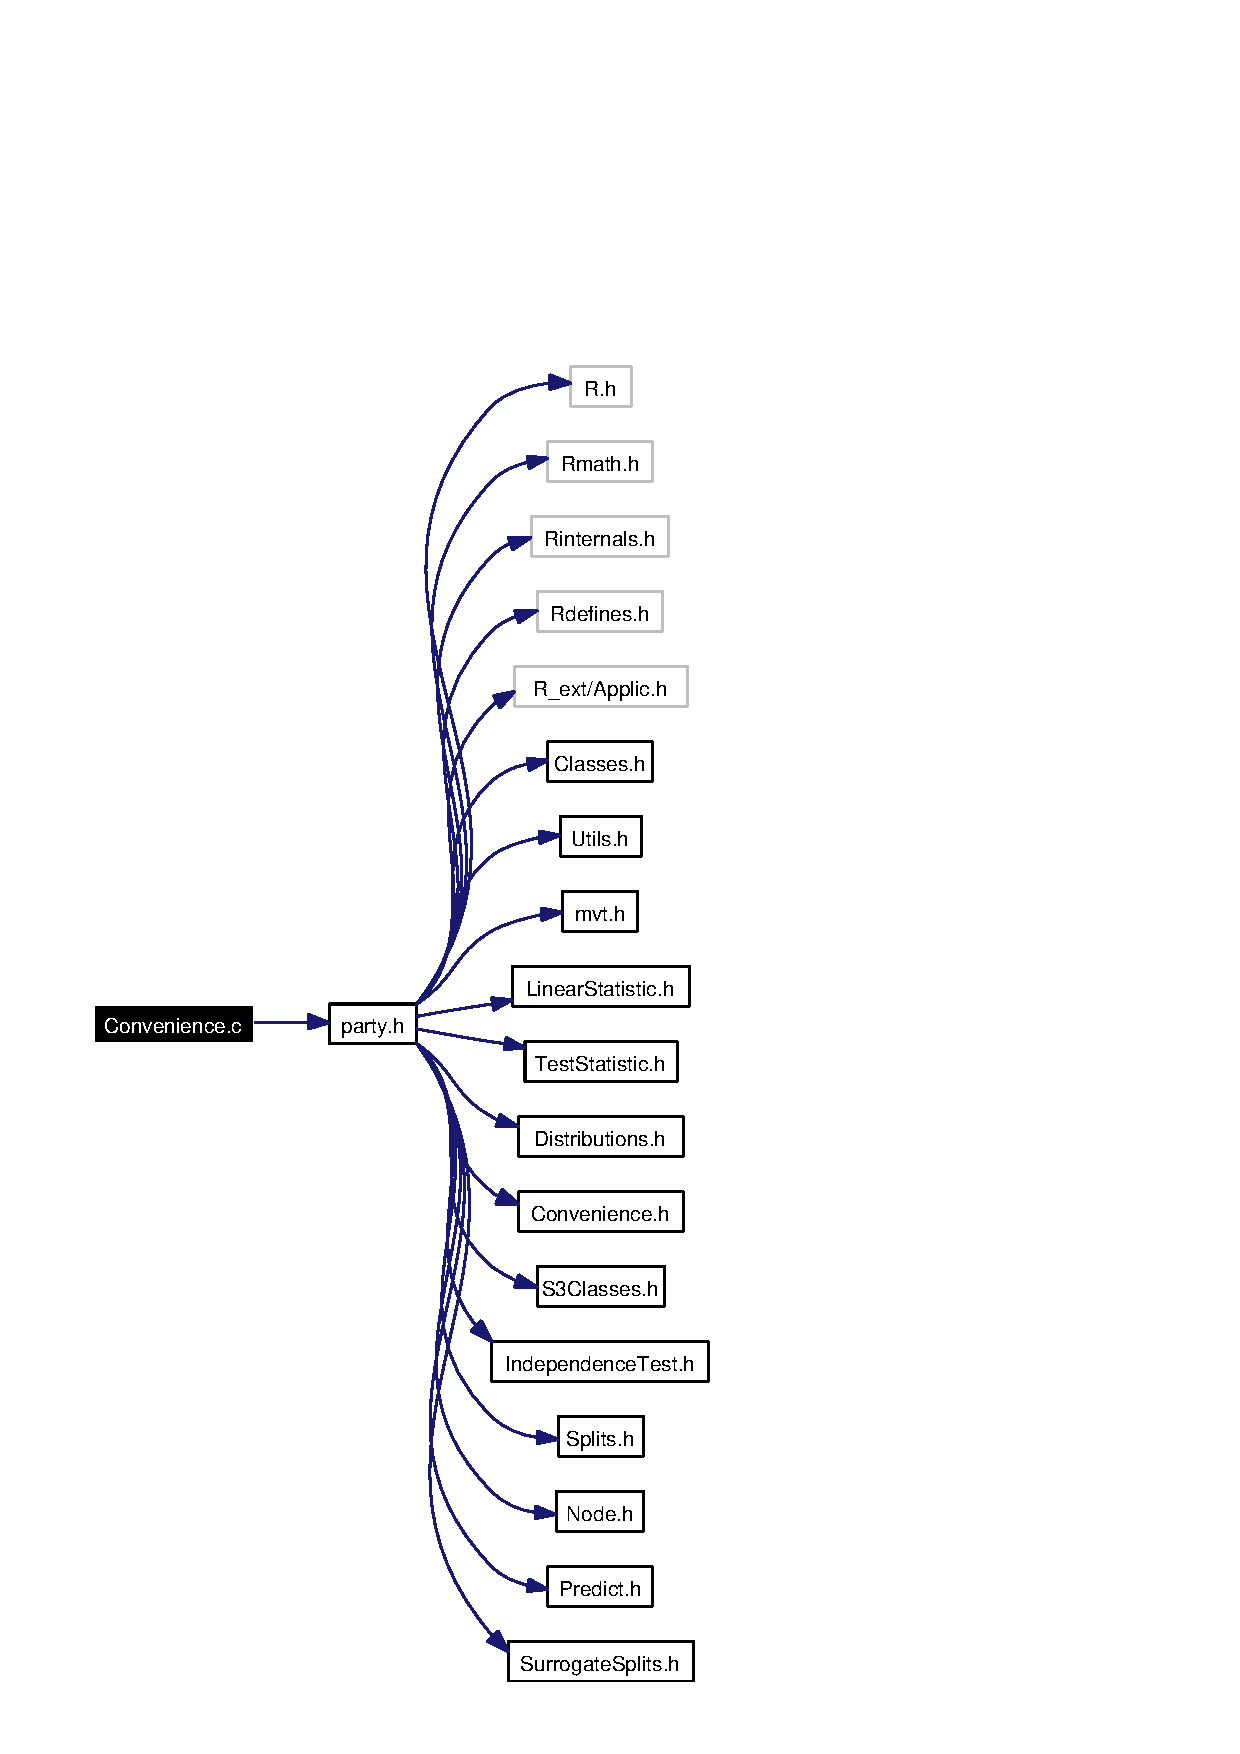
\includegraphics[width=420pt]{Convenience_8c__incl}
\end{center}
\end{figure}
\subsection*{Functions}
\begin{CompactItemize}
\item 
void \hyperlink{Convenience_8c_8d5dcca68051449e29f3b857d375c4a0}{C\_\-LinStatExpCov} (const double $\ast$x, const int p, const double $\ast$y, const int q, const double $\ast$weights, const int n, const int cexpcovinf, SEXP expcovinf, SEXP ans)
\item 
void \hyperlink{Convenience_8c_f39bdd14f23726fdd6bf74888ffbf920}{C\_\-LinStatExpCovMPinv} (SEXP linexpcov, double tol)
\item 
double \hyperlink{Convenience_8c_26159cd74cebf8ff7073ff588864e9ab}{C\_\-TestStatistic} (const SEXP linexpcov, const int type, const double tol)
\item 
double \hyperlink{Convenience_8c_a1bfc91db235a3a166a39ed1e0a224d7}{C\_\-ConditionalPvalue} (const double tstat, SEXP linexpcov, const int type, double tol, int $\ast$maxpts, double $\ast$releps, double $\ast$abseps)
\item 
SEXP \hyperlink{Convenience_8c_5253d5c6a188d9b7a1318c91d958047d}{R\_\-get\_\-response} (SEXP learnsample)
\item 
void \hyperlink{Convenience_8c_a1e8edb4fa73a26e73bc153c45a867b0}{R\_\-set\_\-response} (SEXP learnsample, SEXP y)
\end{CompactItemize}


\subsection{Detailed Description}
Some convenience functions

\begin{Desc}
\item[Author:]\end{Desc}
\begin{Desc}
\item[Author]hothorn \end{Desc}
\begin{Desc}
\item[Date:]\end{Desc}
\begin{Desc}
\item[Date]2008-10-15 11:04:00 +0200 (Wed, 15 Oct 2008) \end{Desc}


Definition in file \hyperlink{Convenience_8c-source}{Convenience.c}.

\subsection{Function Documentation}
\hypertarget{Convenience_8c_a1bfc91db235a3a166a39ed1e0a224d7}{
\index{Convenience.c@{Convenience.c}!C\_\-ConditionalPvalue@{C\_\-ConditionalPvalue}}
\index{C\_\-ConditionalPvalue@{C\_\-ConditionalPvalue}!Convenience.c@{Convenience.c}}
\subsubsection[C\_\-ConditionalPvalue]{\setlength{\rightskip}{0pt plus 5cm}double C\_\-ConditionalPvalue (const double {\em tstat}, \/  SEXP {\em linexpcov}, \/  const int {\em type}, \/  double {\em tol}, \/  int $\ast$ {\em maxpts}, \/  double $\ast$ {\em releps}, \/  double $\ast$ {\em abseps})}}
\label{Convenience_8c_a1bfc91db235a3a166a39ed1e0a224d7}


Compute asymptotic conditional P-value \begin{Desc}
\item[Parameters:]
\begin{description}
\item[{\em tstat}]test statistic \item[{\em linexpcov}]an object of class `LinStatExpectCovar' \item[{\em type}]integer, 1 (maxabs) or 2 (quadform) \item[{\em tol}]tolerance \item[{\em maxpts}]argument to C\_\-maxabsConditionalPvalue \item[{\em releps}]argument to C\_\-maxabsConditionalPvalue \item[{\em abseps}]argument to C\_\-maxabsConditionalPvalue \end{description}
\end{Desc}


Definition at line 99 of file Convenience.c.

References C\_\-maxabsConditionalPvalue(), C\_\-quadformConditionalPvalue(), get\_\-dimension(), MAXABS, PL2\_\-covarianceSym, PL2\_\-rankSym, and QUADFORM.

Referenced by C\_\-TeststatPvalue().

Here is the call graph for this function:\nopagebreak
\begin{figure}[H]
\begin{center}
\leavevmode
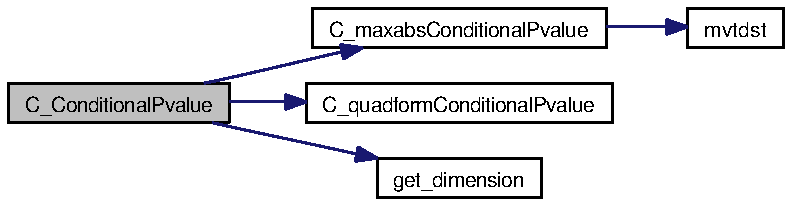
\includegraphics[width=208pt]{Convenience_8c_a1bfc91db235a3a166a39ed1e0a224d7_cgraph}
\end{center}
\end{figure}
\hypertarget{Convenience_8c_8d5dcca68051449e29f3b857d375c4a0}{
\index{Convenience.c@{Convenience.c}!C\_\-LinStatExpCov@{C\_\-LinStatExpCov}}
\index{C\_\-LinStatExpCov@{C\_\-LinStatExpCov}!Convenience.c@{Convenience.c}}
\subsubsection[C\_\-LinStatExpCov]{\setlength{\rightskip}{0pt plus 5cm}void C\_\-LinStatExpCov (const double $\ast$ {\em x}, \/  const int {\em p}, \/  const double $\ast$ {\em y}, \/  const int {\em q}, \/  const double $\ast$ {\em weights}, \/  const int {\em n}, \/  const int {\em cexpcovinf}, \/  SEXP {\em expcovinf}, \/  SEXP {\em ans})}}
\label{Convenience_8c_8d5dcca68051449e29f3b857d375c4a0}


Linear statistic of x, y, and weights and its conditional expectation and covariance \par
 \begin{Desc}
\item[Parameters:]
\begin{description}
\item[{\em x}]values of the transformation \item[{\em p}]dimension of the transformation \item[{\em y}]values of the influence function \item[{\em q}]dimension of the influence function \item[{\em weights}]case weights \item[{\em n}]number of observations \item[{\em cexpcovinf}]logical: recompute exp and cov of the influence fct \item[{\em expcovinf}]an object of class `ExpectCovarInfluence' \item[{\em ans}]return value; an object of class `LinStatExpectCovar' \end{description}
\end{Desc}


Definition at line 26 of file Convenience.c.

References C\_\-ExpectCovarInfluence(), C\_\-ExpectCovarLinearStatistic(), C\_\-LinearStatistic(), and PL2\_\-linearstatisticSym.

Referenced by C\_\-GlobalTest(), C\_\-IndependenceTest(), and R\_\-splitcategorical().

Here is the call graph for this function:\nopagebreak
\begin{figure}[H]
\begin{center}
\leavevmode
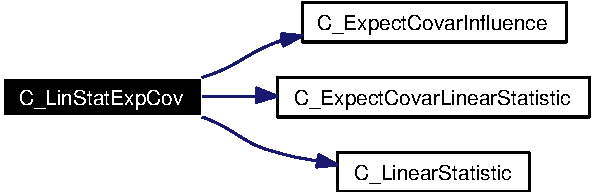
\includegraphics[width=215pt]{Convenience_8c_8d5dcca68051449e29f3b857d375c4a0_cgraph}
\end{center}
\end{figure}
\hypertarget{Convenience_8c_f39bdd14f23726fdd6bf74888ffbf920}{
\index{Convenience.c@{Convenience.c}!C\_\-LinStatExpCovMPinv@{C\_\-LinStatExpCovMPinv}}
\index{C\_\-LinStatExpCovMPinv@{C\_\-LinStatExpCovMPinv}!Convenience.c@{Convenience.c}}
\subsubsection[C\_\-LinStatExpCovMPinv]{\setlength{\rightskip}{0pt plus 5cm}void C\_\-LinStatExpCovMPinv (SEXP {\em linexpcov}, \/  double {\em tol})}}
\label{Convenience_8c_f39bdd14f23726fdd6bf74888ffbf920}


Moore-Penrose inverse of the covariance matrix \par
 \begin{Desc}
\item[Parameters:]
\begin{description}
\item[{\em linexpcov}]an object of class `LinStatExpectCovarMPinv' \item[{\em tol}]tolerance \end{description}
\end{Desc}


Definition at line 46 of file Convenience.c.

References C\_\-MPinv(), PL2\_\-covarianceSym, and PL2\_\-svdmemSym.

Referenced by C\_\-GlobalTest(), and C\_\-IndependenceTest().

Here is the call graph for this function:\nopagebreak
\begin{figure}[H]
\begin{center}
\leavevmode
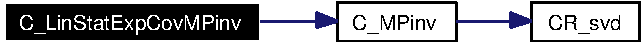
\includegraphics[width=224pt]{Convenience_8c_f39bdd14f23726fdd6bf74888ffbf920_cgraph}
\end{center}
\end{figure}
\hypertarget{Convenience_8c_26159cd74cebf8ff7073ff588864e9ab}{
\index{Convenience.c@{Convenience.c}!C\_\-TestStatistic@{C\_\-TestStatistic}}
\index{C\_\-TestStatistic@{C\_\-TestStatistic}!Convenience.c@{Convenience.c}}
\subsubsection[C\_\-TestStatistic]{\setlength{\rightskip}{0pt plus 5cm}double C\_\-TestStatistic (const SEXP {\em linexpcov}, \/  const int {\em type}, \/  const double {\em tol})}}
\label{Convenience_8c_26159cd74cebf8ff7073ff588864e9ab}


Compute test statistic \begin{Desc}
\item[Parameters:]
\begin{description}
\item[{\em linexpcov}]an object of class `LinStatExpectCovar' \item[{\em type}]integer, 1 (maxabs) or 2 (quadform) \item[{\em tol}]tolerance \end{description}
\end{Desc}


Definition at line 59 of file Convenience.c.

References C\_\-maxabsTestStatistic(), C\_\-quadformTestStatistic(), get\_\-dimension(), PL2\_\-covarianceSym, PL2\_\-expectationSym, PL2\_\-linearstatisticSym, and PL2\_\-MPinvSym.

Referenced by C\_\-TeststatPvalue().

Here is the call graph for this function:\nopagebreak
\begin{figure}[H]
\begin{center}
\leavevmode
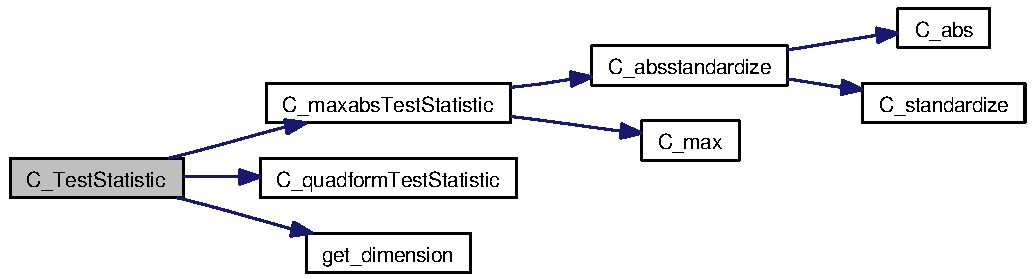
\includegraphics[width=266pt]{Convenience_8c_26159cd74cebf8ff7073ff588864e9ab_cgraph}
\end{center}
\end{figure}
\hypertarget{Convenience_8c_5253d5c6a188d9b7a1318c91d958047d}{
\index{Convenience.c@{Convenience.c}!R\_\-get\_\-response@{R\_\-get\_\-response}}
\index{R\_\-get\_\-response@{R\_\-get\_\-response}!Convenience.c@{Convenience.c}}
\subsubsection[R\_\-get\_\-response]{\setlength{\rightskip}{0pt plus 5cm}SEXP R\_\-get\_\-response (SEXP {\em learnsample})}}
\label{Convenience_8c_5253d5c6a188d9b7a1318c91d958047d}


extract the (first) response variable from a learning sample \begin{Desc}
\item[Parameters:]
\begin{description}
\item[{\em learnsample}]an object of class `LearningSample' \end{description}
\end{Desc}


Definition at line 133 of file Convenience.c.

References PL2\_\-responsesSym, and PL2\_\-variablesSym.

Referenced by R\_\-set\_\-response().\hypertarget{Convenience_8c_a1e8edb4fa73a26e73bc153c45a867b0}{
\index{Convenience.c@{Convenience.c}!R\_\-set\_\-response@{R\_\-set\_\-response}}
\index{R\_\-set\_\-response@{R\_\-set\_\-response}!Convenience.c@{Convenience.c}}
\subsubsection[R\_\-set\_\-response]{\setlength{\rightskip}{0pt plus 5cm}void R\_\-set\_\-response (SEXP {\em learnsample}, \/  SEXP {\em y})}}
\label{Convenience_8c_a1e8edb4fa73a26e73bc153c45a867b0}


change the values of the response variable in a learning sample \begin{Desc}
\item[Parameters:]
\begin{description}
\item[{\em learnsample}]an object of class `LearningSample' \item[{\em y}]a REAL with new values \end{description}
\end{Desc}


Definition at line 145 of file Convenience.c.

References get\_\-predict\_\-trafo(), get\_\-test\_\-trafo(), PL2\_\-responsesSym, PL2\_\-transformationsSym, PL2\_\-variablesSym, and R\_\-get\_\-response().

Here is the call graph for this function:\nopagebreak
\begin{figure}[H]
\begin{center}
\leavevmode
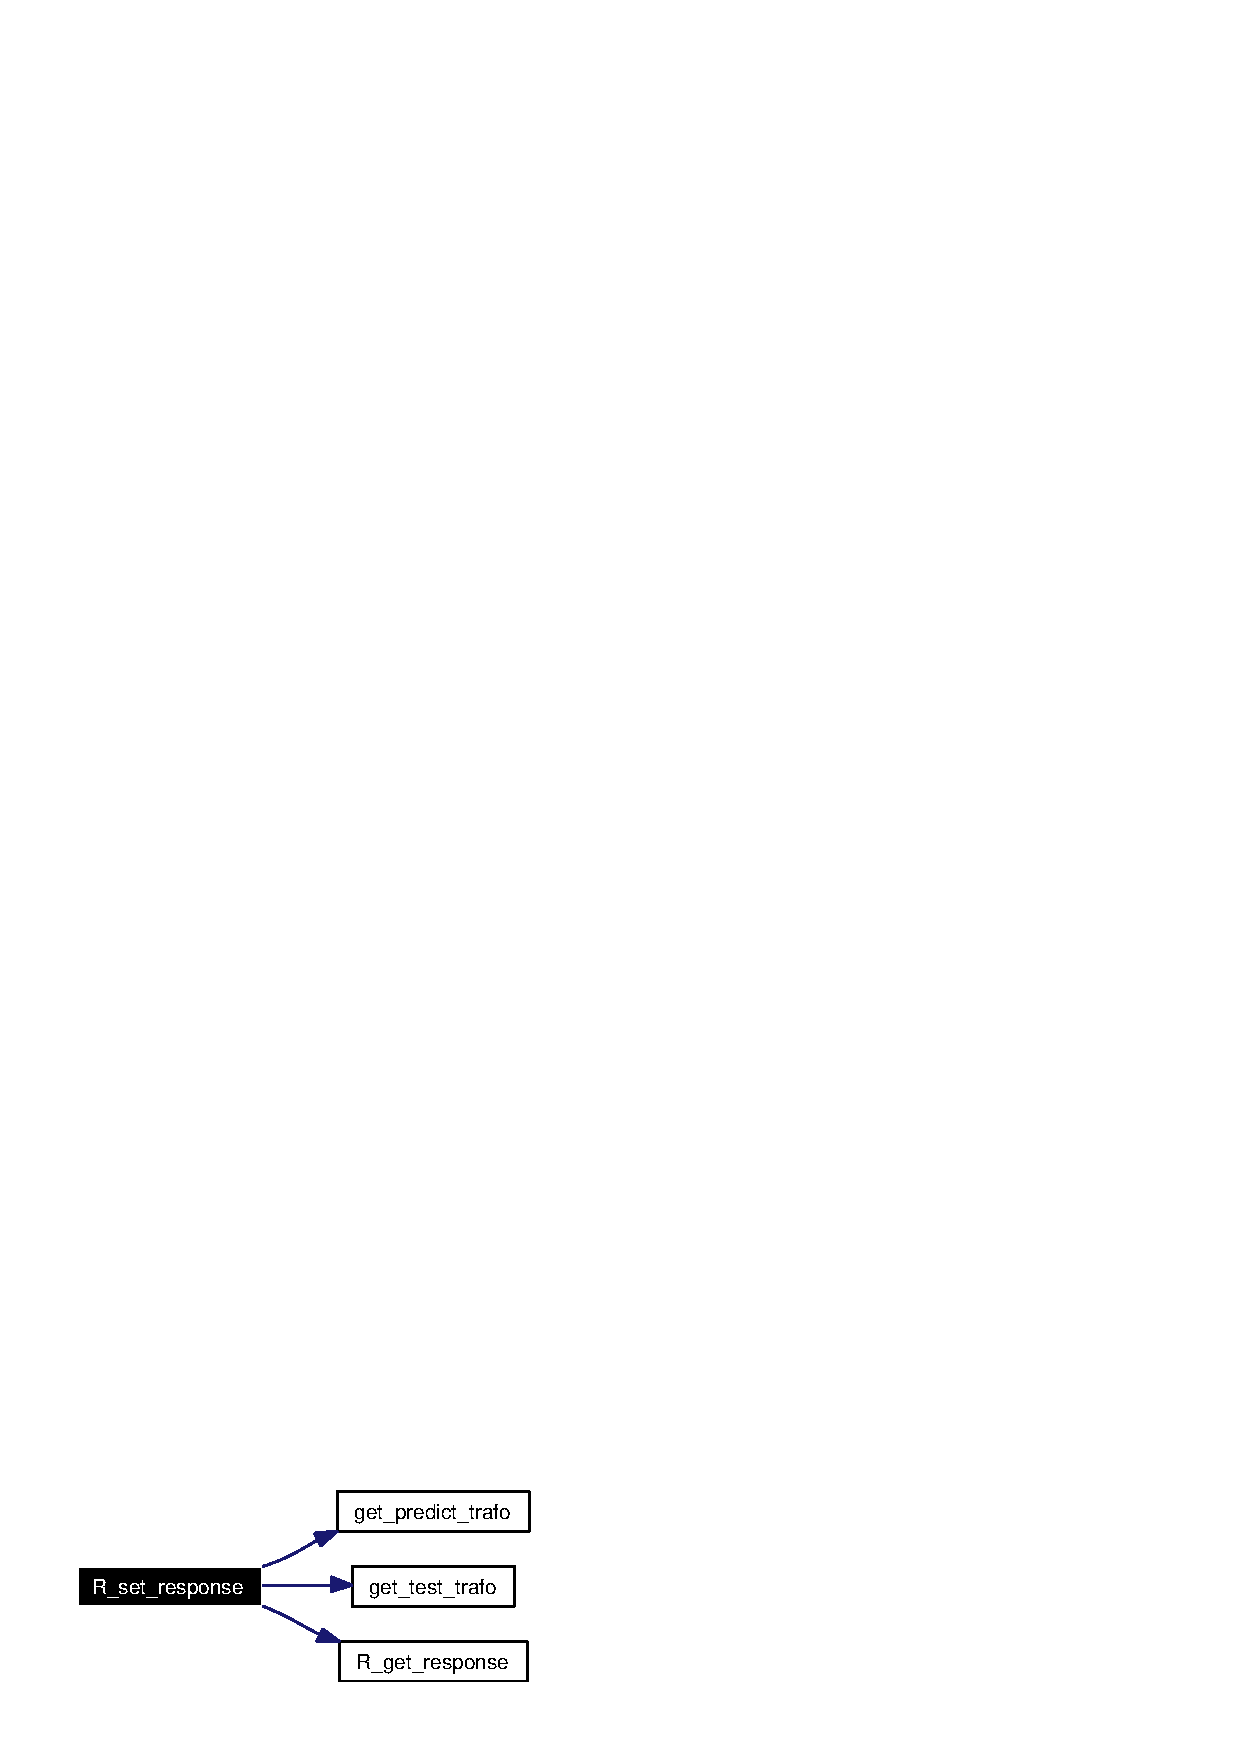
\includegraphics[width=129pt]{Convenience_8c_a1e8edb4fa73a26e73bc153c45a867b0_cgraph}
\end{center}
\end{figure}
